\chapter{Implementation}
\label{chapter:implementation}

The following Sections describe an implementation of the proposed method
described in Chapter \ref{chapter:proposed-method}. This implementation uses the
intuitionistic fuzzy system described in \cite{Hernandez-Aguila2017}, which is
programmed in Clojure (\url{https://github.com/amherag/intuitionistic-fis}), and a
custom-made multi-agent system that was done in Common Lisp
(\url{https://github.com/amherag/neuropredictions}).

\section{Defining the Input Dataset}
\label{section:defining-the-input-dataset}

The dataset to be used must consist of a time series representing the prices
of a financial market. The number of data points needs to be greater than the
number of data points to be used for the preprocessing algorithm (see Section
\ref{section:preprocessing-a-financial-market-using-retracements:implementation}). To
better understand this, consider the scenario where 100 data points are used to
generate the sets of retracements for the price at time $t_0$: none of the first
100 prices in the dataset are useful for the proposed method, as no retracements
can yet be calculated and associated to them due to lack of data. Once the first
100 data points are used to generate the sets of retracements, one can associate
them to the 101st price in the time series.

Although it is common in financial market datasets to provide the open, high,
low and close prices of each of the data points, the current implementation of the
proposed method only uses the close price of each session. For example, in a
dataset consisting of 1 hour sessions, the highest and lowest price achieved in
that hour, and the opening price are discarded, and only the last price recorded
in that hour is used. It is also common to see a volume count in the datasets;
this information is also discarded. Finally, the time associated to each session
in the dataset is used, which means that from any financial market dataset used,
this implementation only uses the close price of each session and the time at
which this close price occurred. Discarding this data does not mean that it is
not useful, as it can be considered in later versions of the implementation;
it is discarded only because it helps to maintain the implementation simple.
% Please justify why, to be more compact? to run the alg. faster? - Mario

This implementation has only been tested with datasets of foreign exchange
financial markets. However, it should work with datasets of other
markets.
% Again, why? - Mario

\section{Preprocessing a Financial Market using Retracements}
\label{section:preprocessing-a-financial-market-using-retracements:implementation}

After a trial and error process in undocumented initial experiments, it was
found convenient to use 20 data points to generate the sets of retracements
associated to each price point. The subjective metrics used to determine this
are the processing time required and the interpretability of the plots generated
with this parameter. %% The author of this thesis used the resulting plots as a
%% guideline to perform a series of successful real trades in multiple foreign
%% exchange markets by opening a trade whenever the price reached low weight
%% price areas. % More detail? - Mario
%% Amaury: Uhh I just removed it. I think I was going to talk more about this,
%% but it is not relevant at all.

The ratios used to calculate the retracements are determined by the beliefs of
the agent preprocessing the raw market data. These ratios are represented by a
vector of a size that can vary from 1 to 6 random real numbers. These random
real numbers have a value that lies in the interval $[0, 2]$. The vector
representing the beliefs varies in size in order to increase the method's
capacity of representing different agent profiles. The size limit of 6 beliefs
was arbitrarily set.

After calculating the sets of retracements for the last 20 price differences,
these are used to determine weighed price areas. Price areas are intervals of
prices of a fixed height, which is 10 asset units in the case of this
implementation. For example, in the case of the Euro vs United States Dollar,
the price interval $[1.1300, 1.1400]$ can be divided into ten price areas of 10
units each, as a single unit in this market is equivalent to $0.0010$. If three
retracement prices are contained in the interval $\left[1.1300, 1.1310\right)$, then
  this area is associated a weight of $3$. An example of such price areas is
  shown in Figure \ref{figure:example-of-retracement-areas}. The heatmap scale
  is shown at the right, showing that blocks with a greater weight are of a
  lighter color, while blocks with a lower weight are of a darker color. In
  further versions of this implementation it should be possible to choose values
  different than 10, but at the moment the implementation only works with powers
  of 10, e.g. 1, 10, 100, 1000, etc. This limitation is due to a bug on how the
  method is coded. Considering the available options for this parameter, 10 is
  the only setting that made sense to use for the timeframe chosen for the
  datasets, as using 1-unit price areas is the equivalent to not using price
  areas at all, and 100-unit and higher price areas would not have an
  appropriate granularity for the 1-hour timeframe, i.e. the agents would end
  perceiving a few number of price areas.
  % Could you explain why 10 units? - Mario 

\begin{figure}
\centering
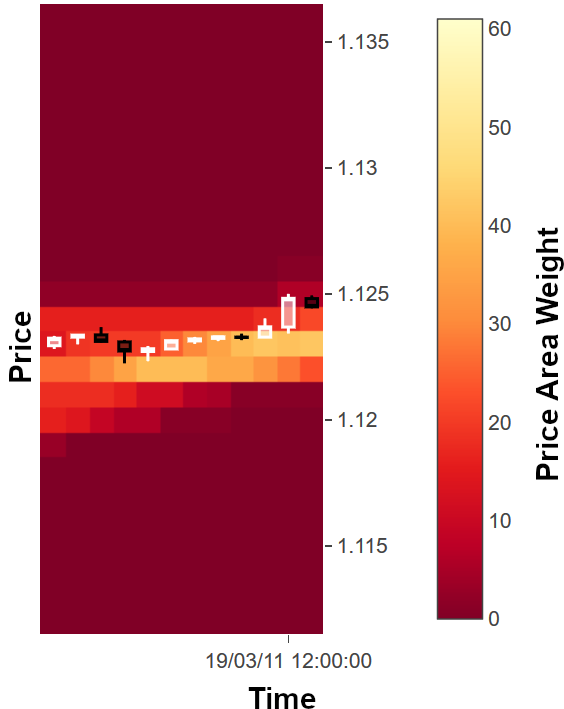
\includegraphics[height=0.6\textwidth]{img/retracement-areas.png}
\caption{Example of retracement areas}
\label{figure:example-of-retracement-areas}
\end{figure}

\section{Using Agents to Represent Traders in a Financial Market}
\label{section:using-agents-to-represent-traders-in-a-financial-market:implementation}

An agent is represented by a vector containing its beliefs and by a matrix
containing its rules. The elements in the belief vector, as mentioned in
\ref{section:defining-the-input-dataset}, are random real numbers with values in
the interval $[0, 2]$ which are later optimized using a genetic algorithm.
% Values in the belief vector continue to be random or
% they are optimized later? Please explain. -Mario

Each of the rules are composed of four elements: three antecedents and one
consequent. Each of these propositions are composed of vectors of three
elements, where the first and second elements are real numbers, with random
values in the interval $[0, 100]$, which represent the means of Gaussian
membership and non-membership functions, respectively. The last element
represents the indeterminacy in the intuitionistic fuzzy set determined by the
membership and non-membership functions. Indeterminacy is represented by a
random real number, which takes a value in the interval $[0, 1]$, influences
both the membership and non-membership in the following way: if the
indeterminacy is equal to $\pi$, then the max membership value in the membership
function is equal to $1 - \pi$, and the max non-membership value in the
non-membership function is equal to $\pi$.

Each of the agents uses their beliefs to create a perception of the market based
on price areas that are associated to a weight that is based on the number of
retracements contained in them, as explained in Section
\ref{section:defining-the-input-dataset}. These price areas are used as inputs
to the agents' rules, which are used to create an intuitionistic fuzzy
system. Specifically, the fuzzy system is going to be fed the weights of three
price areas: the weight of the area above the current price, the weight of area
that is containing the current price, and the weight of the area below the
current price, where the current price is the market price associated to a
particular time in the time series. An example of this situation is depicted in
Figure \ref{figure:areas-for-ifis}, where the current price is represented by
the black candlestick in the middle of the three price areas. The three areas
are associated to an intuitionistic fuzzy set in the rule vector, and the last
intuitionistic fuzzy set is associated to the agent's trade decision, i.e. how
many units is it going to trade for a particular market perception.

\begin{figure}
\centering

\includegraphics[height=0.15\textwidth]{img/areas-for-ifis.png}
\caption{Graphical representation of the price areas used as inputs to the
  intuitionistic fuzzy system}
\label{figure:areas-for-ifis}
\end{figure}

The antecedents of a rule fire the same consequent, and the intersection
operation is applied over the three generated fired consequents (the alpha-cuts
of the consequents). The intersection operation is used to simulate the Boolean
operator \textit{and} among the propositions \cite{Atanassov1986}. After
generating each of the fired -- or alpha-cut -- consequents for each of the rules,
an aggregation is performed using the union operator, which simulates the
consideration of all the rules from an agent. This aggregation process involving
the consequents is described in \ref{eq:aggregation-process}.
% Could the above be stated as a Formula? - Mario 

\begin{equation}
  \label{eq:aggregation-process}
  \bm{A} = \bigcup\limits_{i=1}^{N} \bigcap\limits_{j=1}^{3} \bm{C_{\alpha}}
\end{equation}

The resulting aggregation from the aforementioned process is then
defuzzified using the method found in \cite{Hernandez-Aguila2017} to obtain a
crisp value in the interval $[0, 100]$. In order to be able to simulate sell and
buy orders for the agent, the result of the fuzzy system is then processed by
\ref{eq:agent-trade-units}, which maps the crisp value to a value in the
interval of $[-0.005, 0.005]$ that corresponds to the number of units to buy or
sell.

\begin{equation}
  \label{eq:agent-trade-units}
  A_u(x) = \frac{2x - 100}{10000}
\end{equation}

The number of rules in an agent can vary depending on the desired modelling
capabilities of the system, i.e. an agent with more rules can adopt a more
complex behavior than one with a fewer number of rules. The two drawbacks with
increasing the number of rules are a higher computational cost when optimizinig
the system, and an increased risk of overfitting the system. % I like 'overfitting' more 

Another parameter that can be adjusted in this implementation is the number of
agents in the system. The number of agents, similarly to the number of rules,
can be adjusted depending on the desired modelling capabilities of the system. A
greater number of agents allow the system to achieve a closer curve-fitting to
the real market prices.

\section{Optimization of the Agent-Based Model using a Genetic Algorithm}
\label{section:optimization-of-the-agent-based-model-using-a-genetic-algorithm}

The reader can notice that the implementation already describes 
the necessary components to generate a simulation of a
market. Nevertheless, this simulation will most likely not be a close
resemblance to the real market prices. A genetic algorithm is used to find a
combination of beliefs and rules for the agents that can obtain simulations that
are closer to the real market prices. Genetic algorithms were chosen due to
their simplicity, but the optimization algorithm could easily be changed to
another meta-heuristic.  % Briefly justify the use of a GA - Mario

The genetic algorithm considers an individual or chromosome in two parts: the
beliefs and the rules of the agents. The reason behind this is the
incompatibility between the two data structures; it was considered an easier
approach by the author of the implementation. For example, whenever an agent is
going to suffer a mutation, the mutation algorithm will depend on where it will
occur: either in the beliefs or in the rules segments. In the end, this
differentiation is negligible, but it is noteworthy for the adventurous reader
that wants to examine the implementation provided in its git repository.

As it is noted in the previous paragraph, a single chromosome is composed of
different agents. It is important to remark this, as the reader could be
confused into thinking that a single agent represents an individual or a
chromosome in the genetic algorithm. It can be said that the chromosomes
represent communities of agents. An agent $a$, which is composed
of a set of beliefs $\bm{B}$ and a set of rules $\bm{R}$, create a single
individual $\bm{A}$ in the genetic algorithm. Other representations for this are
depicted in \ref{eq:communities-of-agents} and \ref{eq:communities-of-agents-2}.
% Why not representing the above using math notation (tuples, vectors, sets, indixes, etc.) - Mario
% you could also comment on the other option indenpendent optimization

\begin{equation}
  \label{eq:communities-of-agents}
  \begin{split}
    \bm{A} = \{&\{\{b_1, b_2, \ldots, b_i\}, \{r_1, r_2, \ldots, r_j\}\}_1, \\
               &\{\{b_1, b_2, \ldots, b_i\}, \{r_1, r_2, \ldots, r_j\}\}_2, \\
               &\ldots, \{\{b_1, b_2, \ldots, b_i\}, \{r_1, r_2, \ldots, r_j\}\}_n\}
  \end{split}
\end{equation}

\begin{equation}
  \label{eq:communities-of-agents-2}
  \begin{split}
    \bm{A} &= {(\bm{B_{1}}, \bm{R_{1}}), (\bm{B_{2}}, \bm{R_{2}}), \ldots, (\bm{B_{n}}, \bm{R_{n}})} \\
           &= {a_{1}, a_{2}, \dots, a_{n}}
  \end{split}
\end{equation}

In the following Subsections, the evolutionary process is described in greater
detail.

\subsection{Fitness Function}
\label{subsection:fitness-function}

The fitness of a chromosome is determined by obtaining the mean-squared error
between the agents' simulation of the real market and the real market
prices. This process is described by \ref{eq:mse}, where $R$ is the set of real
market prices, $S$ is the set of simulated market prices and the $MSE$ of both
sets is defined as the squared sum of the differences between each of the real and
simulated prices in the sets. The mean of the result is obtained so the results
are comparable among $MSE$s of price sets of different sizes.

\begin{equation}
  \label{eq:mse}
  MSE(\bm{R}, \bm{S}) = \frac{\sum_{i=1}^n(r_i-s_i)^2}{n}
\end{equation}

The randomly generated communities of agents sometimes throw an error during the
first iterations in the evolutionary process. This is most likely due to
incoherent rules being used to build the intuitionistic fuzzy systems. The way
these cases are handled is by ignoring the error and penalizing these
individuals with a very high error. This way the evolutionary process takes care
of removing buggy individuals. If incoherent rules are indeed being created and
this is the cause of the bug, a way to validate the correctness of the generated
rules could later be added.
% Give a comment between this and havng a way of validating the correctnes of rules before the sim
% Is it too difficult? more time consuming? maybe future work?

\subsection{Selection}
\label{subsection:selection}

Once all the communities of agents in the system are evaluated to obtain their
corresponding error, a process of roulette wheel selection takes place. This
process creates a proportional fitness to each of the communities of agents by
calculating \ref{eq:proportional-fitness}

\begin{equation}
  \label{eq:proportional-fitness}
  p_i = \frac{f_i}{\sum_{j=1}^{N} f_j}
\end{equation}

and this proportional fitness is used to associate a probability of selection to
each community of agents. A random probability of selection in the interval of
$(0, 1.0]$ is generated. If the proportional fitness of a community of agents is
greater than this probability, the individual is chosen, but if this is not the
case, the proportional fitness of that agent is accumulated with the next agent
to be considered for selection, and the process is repeated until a community of
agents with an accumulated proportional fitness greater than the random
probability is found.

The roulette wheel selection algorithm was chosen because it has been suggested
that it works well with both small and medium sized population, in addition to
being a widely used selection algorithm \cite{Hancock2012}
\cite{JinghuiZhong2006}. % Not so much, 
% maybe you could tell this selection is more balanced? It will apear 
% as if everything was arbitrary - Mario


\subsection{Mutation}
\label{subsection:mutation}

After selecting a community of agents using the roulette wheel selection
algorithm, there's a probability of mutation of 0.5\%. The mutation process can
affect an individual in different parts of its constitution, as the
aforementioned mutation probability determines if a gene (a belief or a rule
proposition) should suffer the mutation. This can be seen as a traversal of
every belief and rule in a community of agents, and every time one of the nodes
in this traversal process is visited, there's a chance of modifying the node.

In order to perform the actual mutation, a new random belief value is generated,
in the case of mutating a belief, or a new rule proposition (an antecedent or a
consequent) is generated. The new generated belief or rule proposition then
replaces the belief or rule proposition chosen to be mutated.

Similarly to the roulette wheel selection algorithm, this mutation algorithm was
chosen arbitrarily.

\subsection{Crossover}
\label{subsection:crossover}

The crossover process involves two individuals that recombine their genetic
material which, in this case, represents the beliefs and rules of the agents in
a community of agents. This process is similar to the mutation process, where
there is a probability of occurring.

The crossover is rather simple: all the beliefs of the agents in each of the
community of agents being recombined are concatenated, and then these two
vectors are split at some point, generating four new vectors $A_1$, $A_2$, $B_1$
and $B_2$; the new vector of beliefs for the first community of agents
corresponds to the concatenation of $A_1$ and $B_2$, and the new vector of
beliefs for the second community of agents is obtained by concatenating $B_1$
and $A_2$. This process is then applied to the sets of rules from the two
communities. Algorithm \ref{alg:single-point-crossover} describes the process.

\begin{algorithm}
\caption{Single-point crossover algorithm for two communities of agents}
    \label{alg:single-point-crossover}
\begin{algorithmic}[1]
    
    \Procedure{agents-crossover}{$A, B$};
    \State $bel_A\gets extract\_beliefs(A)$
    \State $bel_B\gets extract\_beliefs(B)$
    
    \State $rul_A\gets extract\_rules(A)$
    \State $rul_B\gets extract\_rules(B)$
    
    \State $bel\_point\gets rand\_int(len(bel_A))$
    \State $rul\_point\gets rand\_int(len(rul_A))$

    \State $bel_{A1}\gets subseq(bel_A, 0, bel\_point)$
    \State $bel_{A2}\gets subseq(bel_A, bel\_point, len(bel_A))$
    \State $bel_{B1}\gets subseq(bel_B, 0, bel\_point)$
    \State $bel_{B2}\gets subseq(bel_B, bel\_point, len(bel_B))$

    \State $rul_{A1}\gets subseq(rul_A, 0, rul\_point)$
    \State $rul_{A2}\gets subseq(rul_A, rul\_point, len(rul_A))$
    \State $rul_{B1}\gets subseq(rul_B, 0, rul\_point)$
    \State $rul_{B2}\gets subseq(rul_B, rul\_point, len(rul_B))$

    \State \textbf{return} $agent(bel_{A1} + bel_{B2}, rul_{A1} + rul_{B2}),
    agent(bel_{B1} + bel_{A2}, rul_{B1} + rul_{A2})$
    \EndProcedure
\end{algorithmic}
\end{algorithm}

This crossover algorithm is commonly known as single-point crossover and it was
chosen due to its simplicity.

% Please add an Algorithm of the above. 
% Use some LaTeX package for this  
% https://tex.stackexchange.com/questions/229355/algorithm-algorithmic-algorithmicx-algorithm2e-algpseudocode-confused 

\subsection{Evolutionary Process}
\label{subsection:evolutionary-process}

The evolutionary process contains all of the processes mentioned in the previous
Subsections. This process is performed for a number of iterations, which are
commonly called generations due to the analogy with biology evolution, and for a
number of communities of agents, which is called a population. The higher the
number of generations, the higher the probability of achieving an individual
with a better fitness.

A generation consists of the following steps: two individuals are selected from
the population, with a probability of suffering a mutation process when
selected, and the crossover process is tried to be applied on them, if the
crossover process is applied, then the two selected individuals will be
recombined, and if it fails the two individuals are returned to the population
unchanged. This process is repeated a number of times equal to the number of
generations.

As an additional step, if the best individual from the previous generation is
recombined with another, a copy of this individual is made and is added to the
population. This is done with the goal of achieving elitism in the evolutionary
process. In order to preserve the size of the population across all the
generations, when the best individual is copied onto the next generation, the
worst individual from the population is discarded. However, after analyzing the
experiments provided in Chapter \ref{chapter:experiments-and-results}, it was
seen that the evolutionary process was not elitist. The reason was later found
to be the order in which the mutation process is performed; once the best
individual is copied onto the next generation's population, the mutation process
is performed.
